\documentclass[../main.tex]{subfiles}

\graphicspath{{../images/}}

\usepackage[noend]{algpseudocode} % for pseudocode
\usepackage[plain]{algorithm} % float environment for algorithms
% preferred pseudocode style
\algrenewcommand{\algorithmicprocedure}{}
\algrenewcommand{\algorithmicthen}{}

% ``do { ... } while (cond)''
\algdef{SE}[DOWHILE]{Do}{doWhile}{\algorithmicdo}[1]{\algorithmicwhile\ #1}%

% ``for (x in y ... z)''
\newcommand{\ForRange}[3]{\For{#1 \textbf{in} #2 \ \ldots \ #3}}

\begin{document}
\pagestyle{fancy}
\chead{Extra Credit}
\rhead{Junseo Shin}
\lhead{CSE 4059}


\renewcommand{\thefigure}{\arabic{figure}}
\section*{COSMIC OpenGL Spacetime Metric in CUDA (COSMIC)}

\begin{figure*}
    \centering
    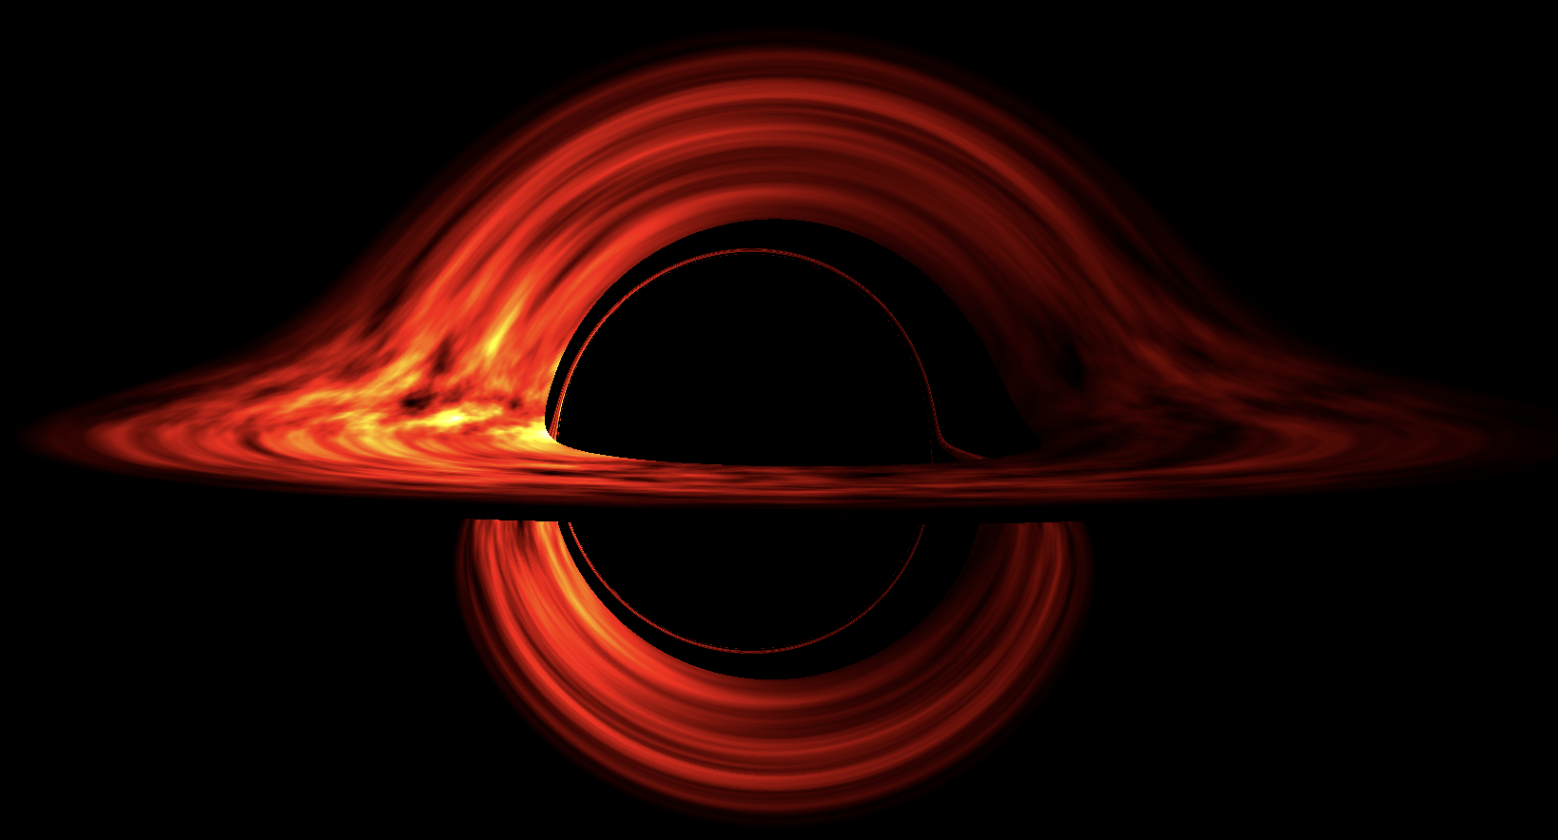
\includegraphics[width=0.75\textwidth]{black_hole.png}
    % set caption width to 0.75\textwidth
    \captionsetup{width=0.75\textwidth}
    \caption{1920x1080 resolution black hole simulation with
    spin $a = 0.99$ and mass $M = 1$. With GPU acceleration via
    CUDA the simulation can be rendered in roughly 4.88 seconds,
    while a single threaded CPU implementation takes up to an hour to render.}
    \label{fig:listscan}
\end{figure*}

The main goal of this project was to use the CUDA programming model to
accelerate the simulation of a black hole. The main bottleneck of the simulation
is that for each pixel on the output image the CPU has to solve a system ordinary
differential equations (ODE) for a photon that is backwards path traced from the
observer and compute the intensity of the light if the photon hits the black hole's
accretion disk \cite{komissarov} \cite{macdonald}. If the photon misses the disk,
or falls into the black hole, we can ignore its contribution to the light intensity,
otherwise we take the normalized photon intensity and account for the gravitational lensing
and Doppler effect as described by Luminet \cite{luminet}.

This simple yet computationally intensive simulation outlines an embarrassingly parallel
problem where larger images can be computed much faster than a sequential
CPU implementation. In order to turn the CPU implementation into GPU code, I had
to first change the data structures to be more GPU friendly via using array pointers
instead of the C++ STL vector class. After the long and tedious process of
writing classes and functions to handle objects that can be instantiated on the GPU for
computing the metric (using the mass and spin of the black hole to compute several matrix
compuations), I wrote a kernel function that dispatches a thread for each pixel in the image,
and compute the light intensity for that pixel.

For very small images (160x90 resolution), the CPU implementation is already quite fast
at rendering the image in 4.79 seconds with multithreading aided by OpenMP
(24 threads on a AMD Ryzen 9 5900X CPU running with max clock speed of 4.95 GHz), but the
GPU implementation embarrassingly outperforms the CPU implementation with a time of 60 milliseconds
which is a 79x speedup. Scaling this up to a 1920x1080 resolution image, the CPU implementation
takes roughly 8 minutes to render the image, while the GPU acceleration takes 4.88 seconds which
is roughly the same time it takes the CPU to render a 160x90 image.

In order to optimize the GPU to run as fast as it could, I had to additionally change the data
type to float as the GPU is optimized for single precision floating point operations. Furthermore,
I used constant memory for the parameters of the black hole, camera position, and the RK45
(Dormand-Prince) ODE solver. Finally I used the hardware defined math instrinsics such as
\texttt{\_\_fsqrt\_rn}, \texttt{\_\_powf}, and \texttt{\_\_fmul\_rn} to double the performance 
of the GPU without adding any numerical imprecision visible in the final image.

Finally, I implemented a simple OpenGL window to display the image using the defined OpenGL
interopability API \texttt{<cuda\_gl\_interop.h>} which maps graphics resources through special
graphics interopability functions such as \texttt{cudaGraphicsMapResources} and transfer the image
data from memory allocated on the device and copies it over to a PBO (pixel buffer object)
defined in the OpenGL context after the kernel execution. This made it so that rendering multiple
frames of the simulation was viewable after each frame was rendered without the computational
overhead of copying the image data back to the CPU and then writing it to a \texttt{.ppm} file.

\subsection*{Source Code: \url{https://github.com/joonsuuh/cosmic}}

The project is built using CMake with several dependencies for OpenGL, CUDA, and OpenMP to
run each of the simulations. There are 4 main executable targets:
\begin{itemize}
    \item \texttt{cosmic\_cpu}: A CPU implementation of the black hole simulation.
    \item \texttt{cosmic\_gpu}: A simple GPU implementation of the black hole simulation.
    \item \texttt{cosmic\_cpu\_gl}: The CPU implementation with OpenGL context window.
    \item \texttt{cosmic\_gpu\_gl}: The CUDA OpenGL interopability with perlin noise to simulate
    an asthetic accretion disk which can be converted from \texttt{.ppm} to \texttt{.mp4} using
    \texttt{FFmpeg} with the provided bash script.
\end{itemize}

% Direct bibliography entries
\begin{thebibliography}{9} % The '9' determines the width allocated for the reference numbers
\bibitem{komissarov} Komissarov, S. S. 2004, Monthly Notices of the Royal Astronomical Society,
350, 427, \href{http://doi.org/10.1111/j.1365-2966.2004.07598.x}{doi: 10.1111/j.1365-2966.2004.07598.x}
\bibitem{macdonald} MacDonald, D., \& Thorne, K. S. 1982, Monthly Notices of the Royal Astronomical Society, 198, 345,
\href{http://doi.org/10.1093/mnras/198.2.345}{doi: 10.1093/mnras/198.2.345}
\bibitem{luminet} Luminet, J. P. 1979, Astronomy and Astrophysics, 75, 228
\end{thebibliography}

\end{document}